% Generated by paper/v2/build_figures.py -- do not edit by hand.
\documentclass[9pt]{extarticle}
\usepackage[paperwidth=21cm,paperheight=29.7cm,textwidth=17.1cm,textheight=26cm,centering]{geometry}
\usepackage[T1]{fontenc}
\usepackage{lmodern}
\usepackage{graphicx}
\usepackage[labelfont=bf,font=small,justification=raggedright,singlelinecheck=false]{caption}
\usepackage[labelformat=parens,labelfont=bf,font=footnotesize,justification=centering]{subcaption}
\usepackage{newunicodechar}
\newunicodechar{±}{\ensuremath{\pm}}
\newunicodechar{°}{\ensuremath{^\circ}}
\newunicodechar{−}{\ensuremath{-}}
\newunicodechar{→}{\ensuremath{\rightarrow}}
\newunicodechar{µ}{\ensuremath{\mu}}
\newunicodechar{μ}{\ensuremath{\mu}}
\newunicodechar{×}{\ensuremath{\times}}
\newunicodechar{≈}{\ensuremath{\approx}}
\newunicodechar{†}{\ensuremath{^\dagger}}
\usepackage{array,booktabs}
\usepackage[hidelinks]{hyperref}
\newcommand{\siref}[1]{S\ref{#1}}
\setlength{\parindent}{0pt}
\pagestyle{empty}
\begin{document}
\begin{figure*}[p]
\centering
\begin{subfigure}[b]{3.450in}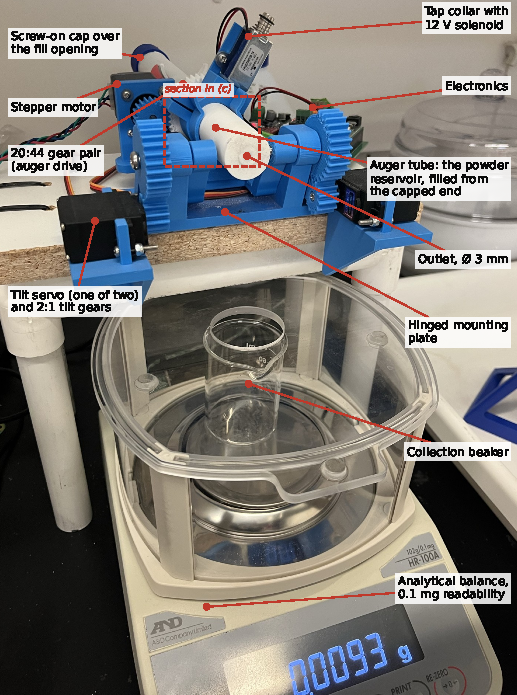
\includegraphics{figures/doser_a_photo.pdf}\caption{As tested}\end{subfigure}\hfill
\begin{minipage}[b]{3.182in}
\begin{subfigure}[b]{\linewidth}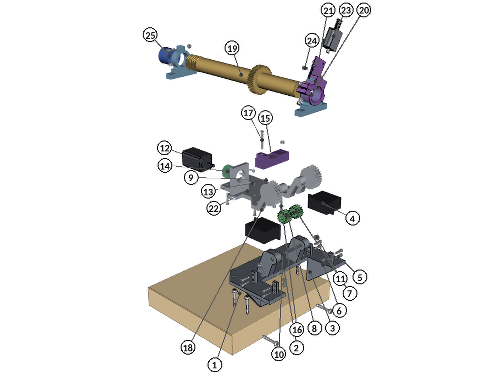
\includegraphics{figures/doser_b_exploded.pdf}\caption{Exploded view}\end{subfigure}\\[6pt]
\begin{subfigure}[b]{1.520in}\centering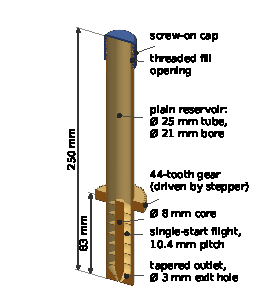
\includegraphics{figures/doser_c_auger.pdf}\caption{Auger section}\end{subfigure}\hfill
\begin{subfigure}[b]{1.644in}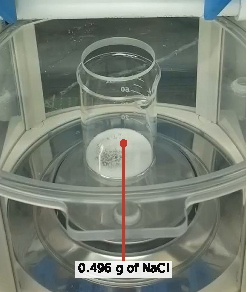
\includegraphics{figures/doser_d_cam.pdf}\caption{Fixed camera}\end{subfigure}
\end{minipage}
\stepcounter{figure}
\end{figure*}
\clearpage
\begin{figure*}[p]
\centering
\begin{subfigure}[b]{\textwidth}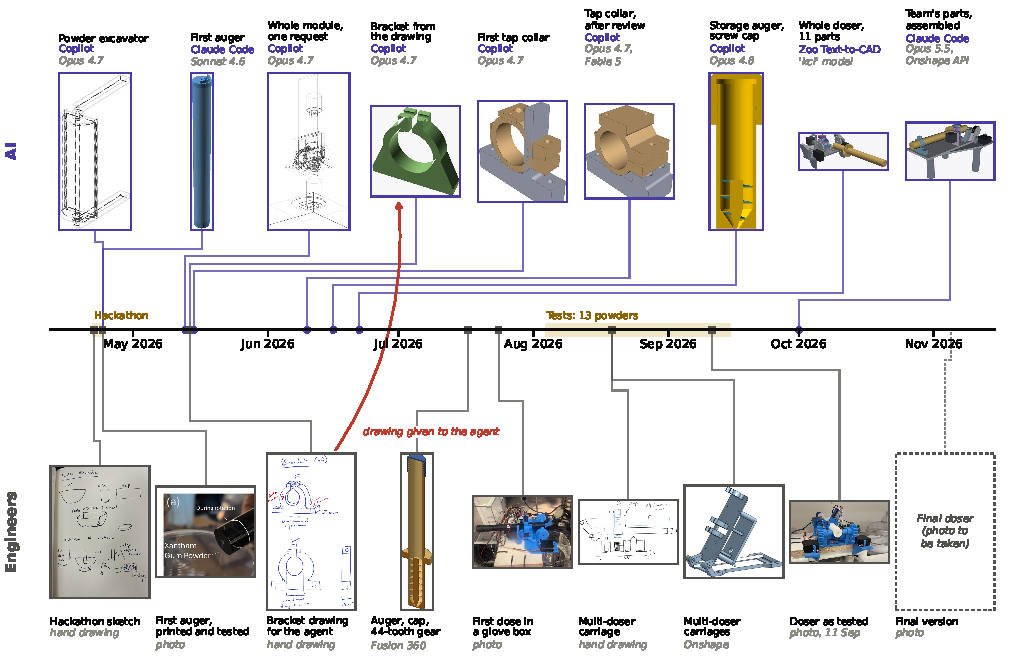
\includegraphics{figures/timeline_a.pdf}\caption{Designs over time}\end{subfigure}\\[4pt]
\begin{subfigure}[b]{\textwidth}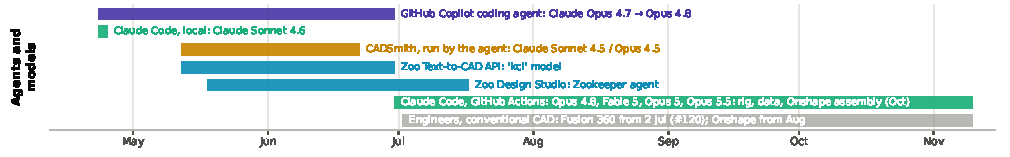
\includegraphics{figures/timeline_b_band.pdf}\caption{Agents and models}\end{subfigure}
\stepcounter{figure}
\end{figure*}
\clearpage
\begin{figure*}[p]
\centering
\begin{subfigure}[b]{\textwidth}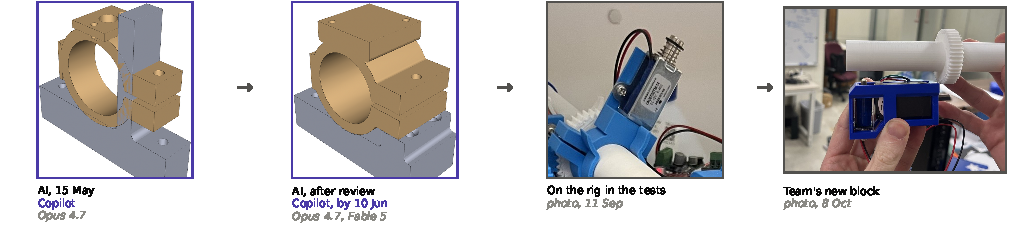
\includegraphics{figures/redesign_a_tapcollar.pdf}\caption{Tap collar}\end{subfigure}\\[6pt]
\begin{subfigure}[b]{2.350in}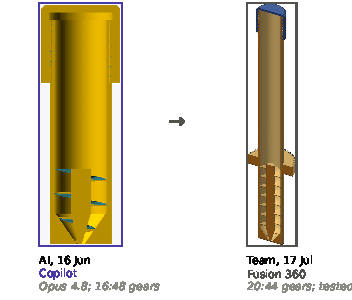
\includegraphics{figures/redesign_b_auger.pdf}\caption{Auger}\end{subfigure}\hfill
\begin{subfigure}[b]{4.150in}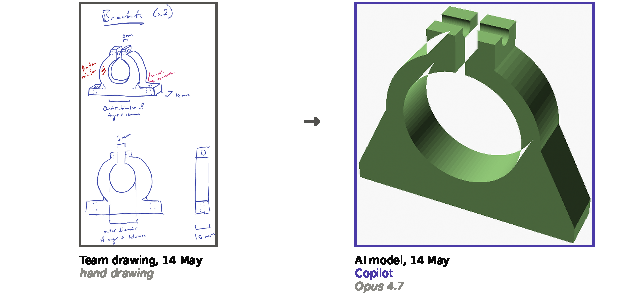
\includegraphics{figures/redesign_c_bracket.pdf}\caption{Bracket}\end{subfigure}
\stepcounter{figure}
\end{figure*}
\clearpage
\begin{figure*}[p]
\centering
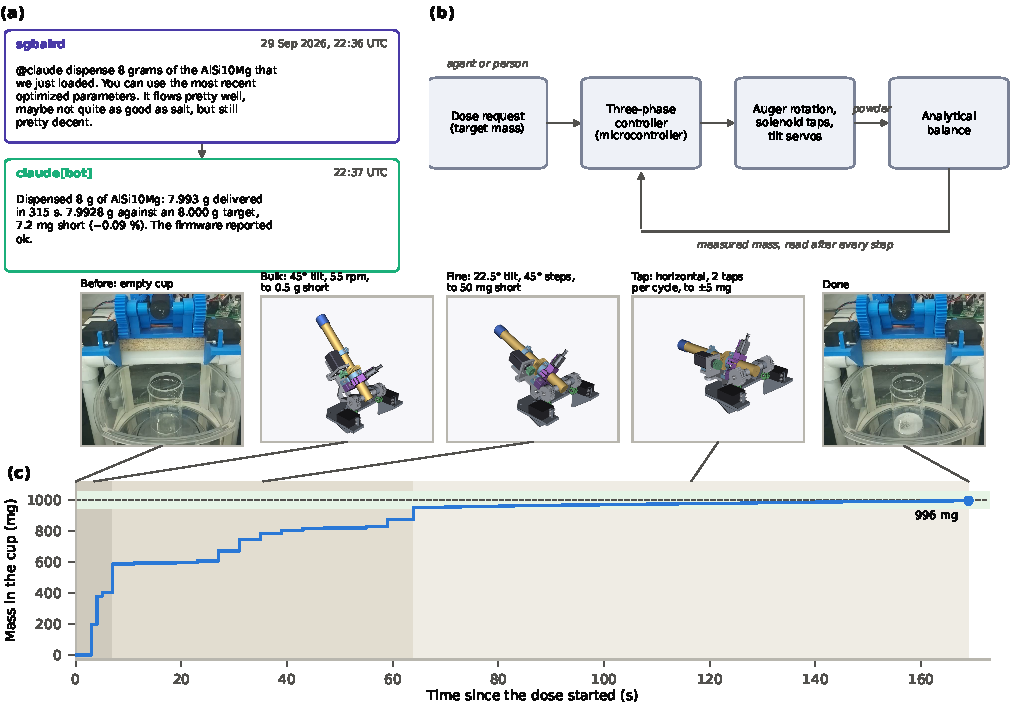
\includegraphics{figures/dosing.pdf}
\stepcounter{figure}
\end{figure*}
\clearpage
\begin{figure*}[p]
\centering
\begin{subfigure}[b]{1.184in}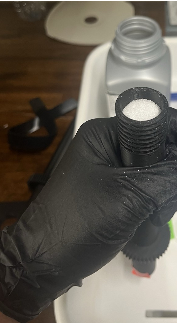
\includegraphics{figures/use_a_fill.pdf}\caption{Fill}\end{subfigure}\hfill\raisebox{1.1in}{$\rightarrow$}\hfill
\begin{subfigure}[b]{1.262in}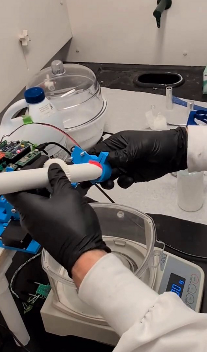
\includegraphics{figures/use_b_fit.pdf}\caption{Fit}\end{subfigure}\hfill\raisebox{1.1in}{$\rightarrow$}\hfill
\begin{subfigure}[b]{1.260in}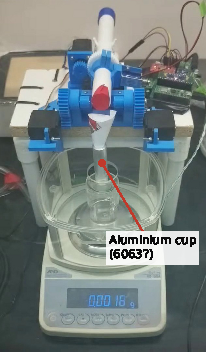
\includegraphics{figures/use_c_ready.pdf}\caption{Over the cup}\end{subfigure}\hfill
\begin{subfigure}[b]{2.751in}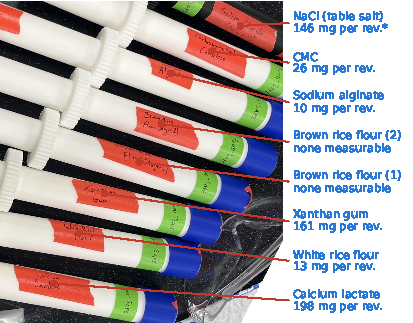
\includegraphics{figures/use_d_augers.pdf}\caption{One auger per powder}\end{subfigure}
\stepcounter{figure}
\end{figure*}
\clearpage
\begin{figure*}[p]
\centering
\begin{subfigure}[b]{2.620in}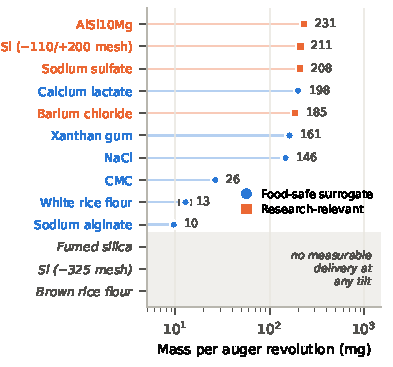
\includegraphics{figures/openloop_a_rev.pdf}\caption{Per revolution}\end{subfigure}\hfill
\begin{subfigure}[b]{1.800in}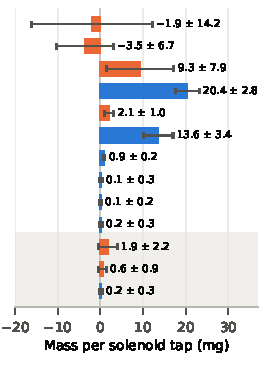
\includegraphics{figures/openloop_b_tap.pdf}\caption{Per tap}\end{subfigure}\hfill
\begin{subfigure}[b]{2.020in}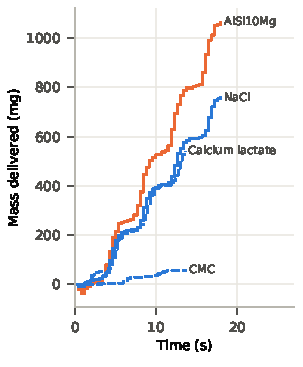
\includegraphics{figures/openloop_c_time.pdf}\caption{In time}\end{subfigure}
\stepcounter{figure}
\end{figure*}
\clearpage
\begin{figure*}[p]
\centering
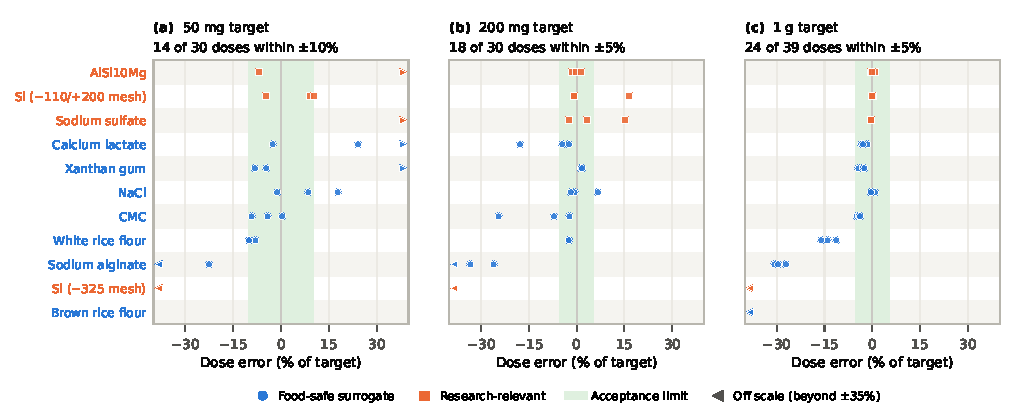
\includegraphics{figures/closedloop.pdf}
\stepcounter{figure}
\end{figure*}
\clearpage
\setcounter{figure}{0}
\begin{figure*}[p]
\centering
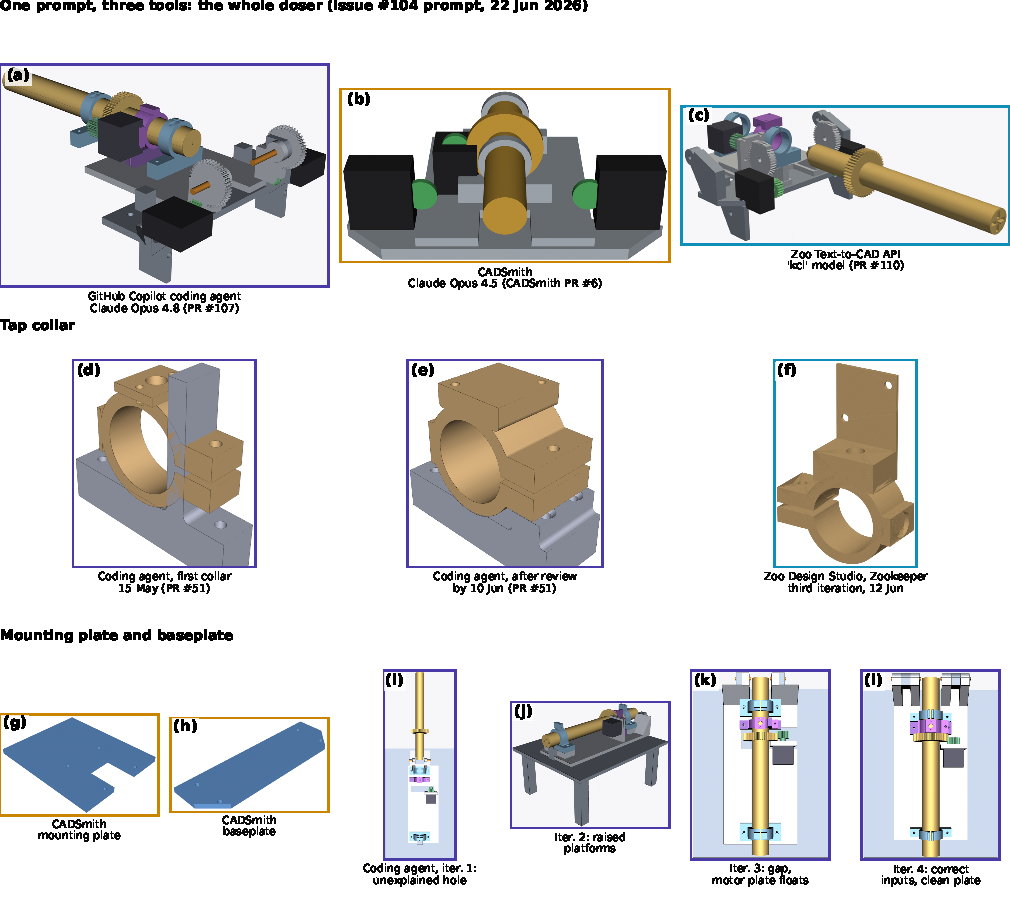
\includegraphics{figures/figS_cad_comparison.pdf}
\stepcounter{figure}
\end{figure*}
\clearpage
\begin{figure*}[p]
\centering
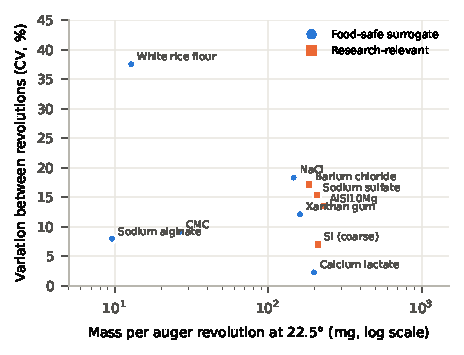
\includegraphics{figures/figS_rev_variation.pdf}
\stepcounter{figure}
\end{figure*}
\clearpage
\begin{figure*}[p]
\centering
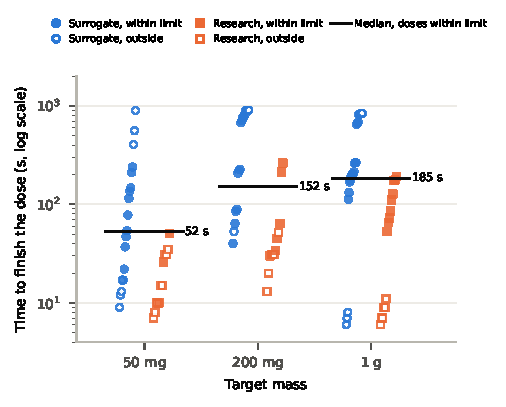
\includegraphics{figures/figS_dose_time.pdf}
\stepcounter{figure}
\end{figure*}
\clearpage
\end{document}
